\documentclass[1p]{elsarticle_modified}
%\bibliographystyle{elsarticle-num}

%\usepackage[colorlinks]{hyperref}
%\usepackage{abbrmath_seonhwa} %\Abb, \Ascr, \Acal ,\Abf, \Afrak
\usepackage{amsfonts}
\usepackage{amssymb}
\usepackage{amsmath}
\usepackage{amsthm}
\usepackage{scalefnt}
\usepackage{amsbsy}
\usepackage{kotex}
\usepackage{caption}
\usepackage{subfig}
\usepackage{color}
\usepackage{graphicx}
\usepackage{xcolor} %% white, black, red, green, blue, cyan, magenta, yellow
\usepackage{float}
\usepackage{setspace}
\usepackage{hyperref}

\usepackage{tikz}
\usetikzlibrary{arrows}

\usepackage{multirow}
\usepackage{array} % fixed length table
\usepackage{hhline}

%%%%%%%%%%%%%%%%%%%%%
\makeatletter
\renewcommand*\env@matrix[1][\arraystretch]{%
	\edef\arraystretch{#1}%
	\hskip -\arraycolsep
	\let\@ifnextchar\new@ifnextchar
	\array{*\c@MaxMatrixCols c}}
\makeatother %https://tex.stackexchange.com/questions/14071/how-can-i-increase-the-line-spacing-in-a-matrix
%%%%%%%%%%%%%%%

\usepackage[normalem]{ulem}

\newcommand{\msout}[1]{\ifmmode\text{\sout{\ensuremath{#1}}}\else\sout{#1}\fi}
%SOURCE: \msout is \stkout macro in https://tex.stackexchange.com/questions/20609/strikeout-in-math-mode

\newcommand{\cancel}[1]{
	\ifmmode
	{\color{red}\msout{#1}}
	\else
	{\color{red}\sout{#1}}
	\fi
}

\newcommand{\add}[1]{
	{\color{blue}\uwave{#1}}
}

\newcommand{\replace}[2]{
	\ifmmode
	{\color{red}\msout{#1}}{\color{blue}\uwave{#2}}
	\else
	{\color{red}\sout{#1}}{\color{blue}\uwave{#2}}
	\fi
}

\newcommand{\Sol}{\mathcal{S}} %segment
\newcommand{\D}{D} %diagram
\newcommand{\A}{\mathcal{A}} %arc


%%%%%%%%%%%%%%%%%%%%%%%%%%%%%5 test

\def\sl{\operatorname{\textup{SL}}(2,\Cbb)}
\def\psl{\operatorname{\textup{PSL}}(2,\Cbb)}
\def\quan{\mkern 1mu \triangleright \mkern 1mu}

\theoremstyle{definition}
\newtheorem{thm}{Theorem}[section]
\newtheorem{prop}[thm]{Proposition}
\newtheorem{lem}[thm]{Lemma}
\newtheorem{ques}[thm]{Question}
\newtheorem{cor}[thm]{Corollary}
\newtheorem{defn}[thm]{Definition}
\newtheorem{exam}[thm]{Example}
\newtheorem{rmk}[thm]{Remark}
\newtheorem{alg}[thm]{Algorithm}

\newcommand{\I}{\sqrt{-1}}
\begin{document}

%\begin{frontmatter}
%
%\title{Boundary parabolic representations of knots up to 8 crossings}
%
%%% Group authors per affiliation:
%\author{Yunhi Cho} 
%\address{Department of Mathematics, University of Seoul, Seoul, Korea}
%\ead{yhcho@uos.ac.kr}
%
%
%\author{Seonhwa Kim} %\fnref{s_kim}}
%\address{Center for Geometry and Physics, Institute for Basic Science, Pohang, 37673, Korea}
%\ead{ryeona17@ibs.re.kr}
%
%\author{Hyuk Kim}
%\address{Department of Mathematical Sciences, Seoul National University, Seoul 08826, Korea}
%\ead{hyukkim@snu.ac.kr}
%
%\author{Seokbeom Yoon}
%\address{Department of Mathematical Sciences, Seoul National University, Seoul, 08826,  Korea}
%\ead{sbyoon15@snu.ac.kr}
%
%\begin{abstract}
%We find all boundary parabolic representation of knots up to 8 crossings.
%
%\end{abstract}
%\begin{keyword}
%    \MSC[2010] 57M25 
%\end{keyword}
%
%\end{frontmatter}

%\linenumbers
%\tableofcontents
%
\newcommand\colored[1]{\textcolor{white}{\rule[-0.35ex]{0.8em}{1.4ex}}\kern-0.8em\color{red} #1}%
%\newcommand\colored[1]{\textcolor{white}{ #1}\kern-2.17ex	\textcolor{white}{ #1}\kern-1.81ex	\textcolor{white}{ #1}\kern-2.15ex\color{red}#1	}

{\Large $\underline{12a_{1177}~(K12a_{1177})}$}

\setlength{\tabcolsep}{10pt}
\renewcommand{\arraystretch}{1.6}
\vspace{1cm}\begin{tabular}{m{100pt}>{\centering\arraybackslash}m{274pt}}
\multirow{5}{120pt}{
	\centering
	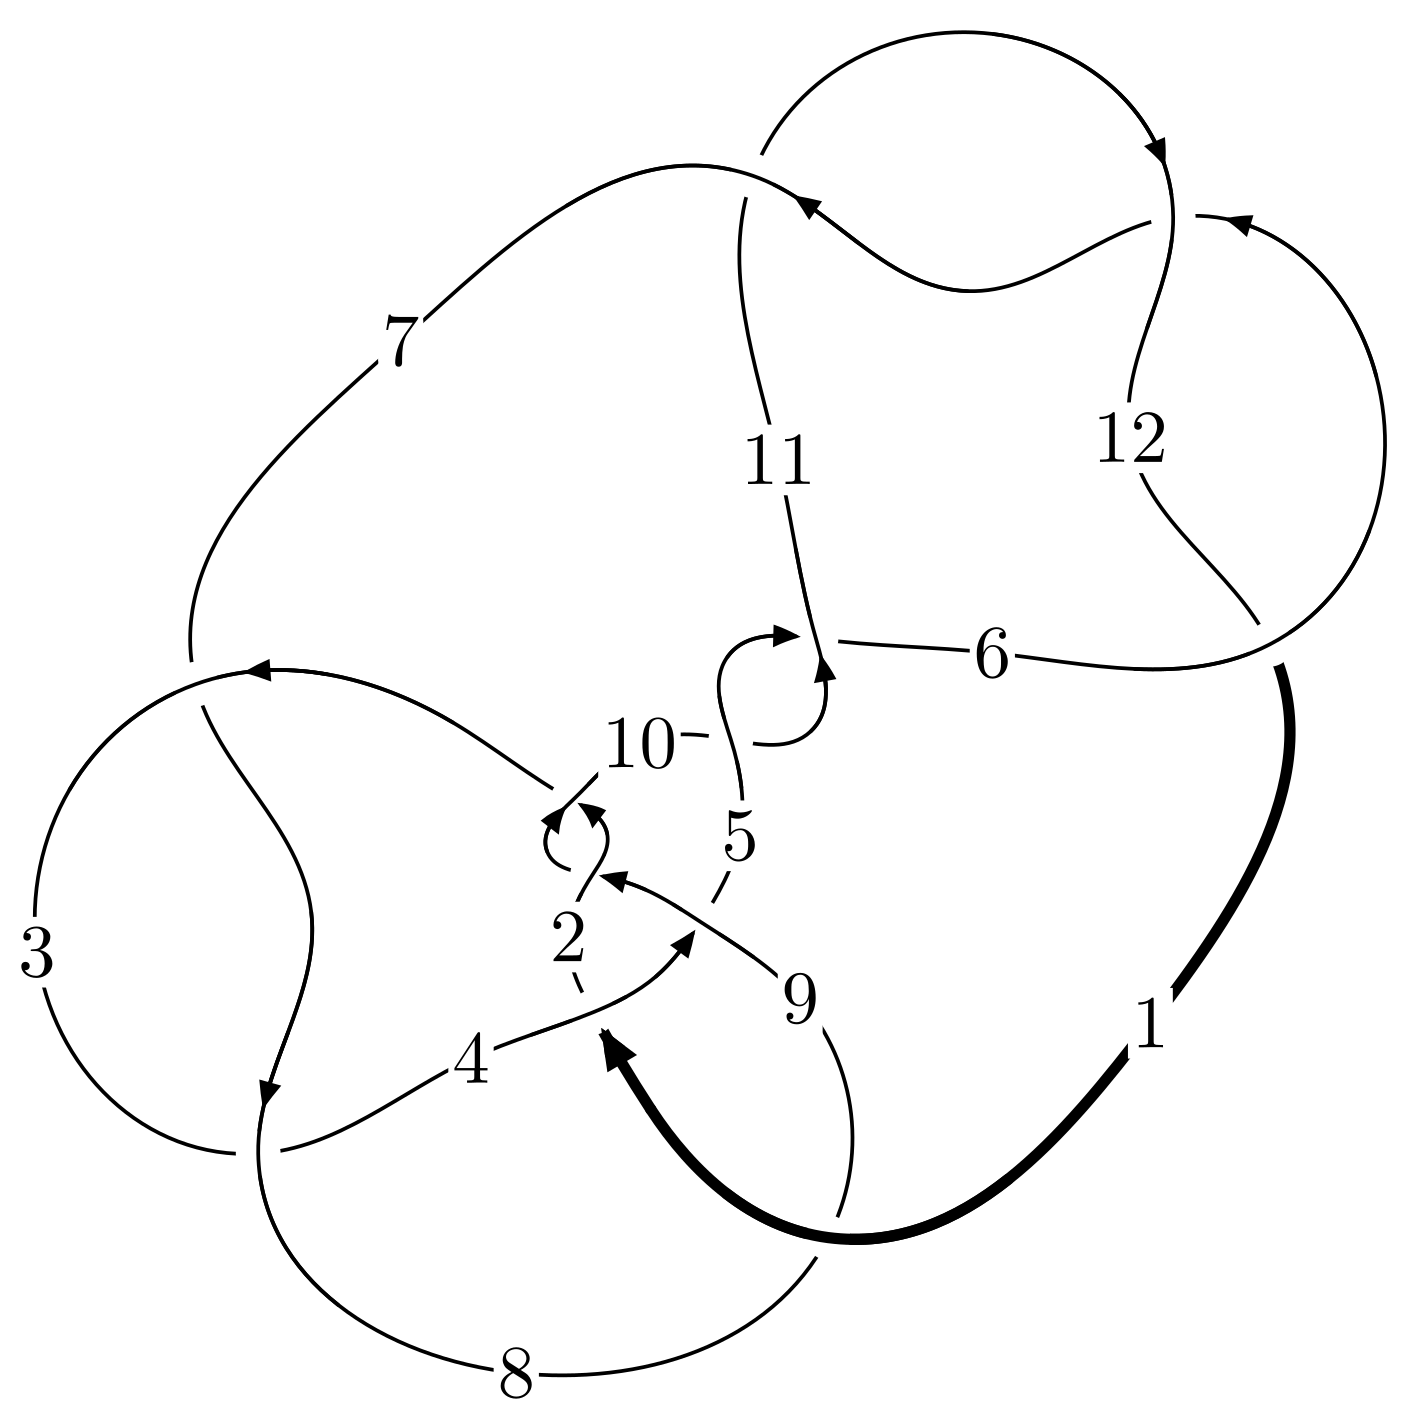
\includegraphics[width=112pt]{../../../GIT/diagram.site/Diagrams/png/1978_12a_1177.png}\\
\ \ \ A knot diagram\footnotemark}&
\allowdisplaybreaks
\textbf{Linearized knot diagam} \\
\cline{2-2}
 &
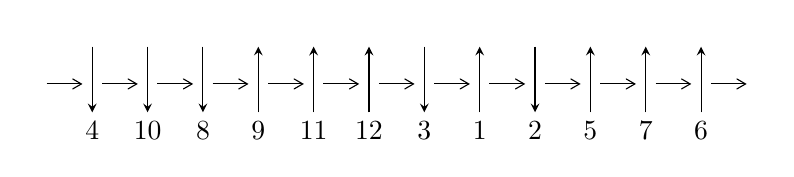
\begin{tikzpicture}[x=20pt, y=17pt]
	% nodes
	\node (C0) at (0, 0) {};
	\node (C1) at (1, 0) {};
	\node (C1U) at (1, +1) {};
	\node (C1D) at (1, -1) {4};

	\node (C2) at (2, 0) {};
	\node (C2U) at (2, +1) {};
	\node (C2D) at (2, -1) {10};

	\node (C3) at (3, 0) {};
	\node (C3U) at (3, +1) {};
	\node (C3D) at (3, -1) {8};

	\node (C4) at (4, 0) {};
	\node (C4U) at (4, +1) {};
	\node (C4D) at (4, -1) {9};

	\node (C5) at (5, 0) {};
	\node (C5U) at (5, +1) {};
	\node (C5D) at (5, -1) {11};

	\node (C6) at (6, 0) {};
	\node (C6U) at (6, +1) {};
	\node (C6D) at (6, -1) {12};

	\node (C7) at (7, 0) {};
	\node (C7U) at (7, +1) {};
	\node (C7D) at (7, -1) {3};

	\node (C8) at (8, 0) {};
	\node (C8U) at (8, +1) {};
	\node (C8D) at (8, -1) {1};

	\node (C9) at (9, 0) {};
	\node (C9U) at (9, +1) {};
	\node (C9D) at (9, -1) {2};

	\node (C10) at (10, 0) {};
	\node (C10U) at (10, +1) {};
	\node (C10D) at (10, -1) {5};

	\node (C11) at (11, 0) {};
	\node (C11U) at (11, +1) {};
	\node (C11D) at (11, -1) {7};

	\node (C12) at (12, 0) {};
	\node (C12U) at (12, +1) {};
	\node (C12D) at (12, -1) {6};
	\node (C13) at (13, 0) {};

	% arrows
	\draw[->,>={angle 60}]
	(C0) edge (C1) (C1) edge (C2) (C2) edge (C3) (C3) edge (C4) (C4) edge (C5) (C5) edge (C6) (C6) edge (C7) (C7) edge (C8) (C8) edge (C9) (C9) edge (C10) (C10) edge (C11) (C11) edge (C12) (C12) edge (C13) ;	\draw[->,>=stealth]
	(C1U) edge (C1D) (C2U) edge (C2D) (C3U) edge (C3D) (C4D) edge (C4U) (C5D) edge (C5U) (C6D) edge (C6U) (C7U) edge (C7D) (C8D) edge (C8U) (C9U) edge (C9D) (C10D) edge (C10U) (C11D) edge (C11U) (C12D) edge (C12U) ;
	\end{tikzpicture} \\
\hhline{~~} \\& 
\textbf{Solving Sequence} \\ \cline{2-2} 
 &
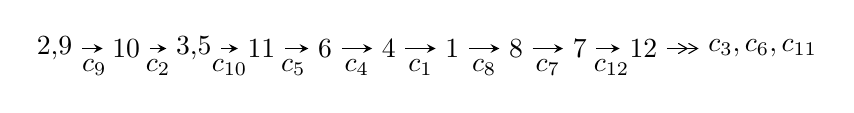
\begin{tikzpicture}[x=23pt, y=7pt]
	% node
	\node (A0) at (-1/8, 0) {2,9};
	\node (A1) at (1, 0) {10};
	\node (A2) at (33/16, 0) {3,5};
	\node (A3) at (25/8, 0) {11};
	\node (A4) at (33/8, 0) {6};
	\node (A5) at (41/8, 0) {4};
	\node (A6) at (49/8, 0) {1};
	\node (A7) at (57/8, 0) {8};
	\node (A8) at (65/8, 0) {7};
	\node (A9) at (73/8, 0) {12};
	\node (C1) at (1/2, -1) {$c_{9}$};
	\node (C2) at (3/2, -1) {$c_{2}$};
	\node (C3) at (21/8, -1) {$c_{10}$};
	\node (C4) at (29/8, -1) {$c_{5}$};
	\node (C5) at (37/8, -1) {$c_{4}$};
	\node (C6) at (45/8, -1) {$c_{1}$};
	\node (C7) at (53/8, -1) {$c_{8}$};
	\node (C8) at (61/8, -1) {$c_{7}$};
	\node (C9) at (69/8, -1) {$c_{12}$};
	\node (A10) at (11, 0) {$c_{3},c_{6},c_{11}$};

	% edge
	\draw[->,>=stealth]	
	(A0) edge (A1) (A1) edge (A2) (A2) edge (A3) (A3) edge (A4) (A4) edge (A5) (A5) edge (A6) (A6) edge (A7) (A7) edge (A8) (A8) edge (A9) ;
	\draw[->>,>={angle 60}]	
	(A9) edge (A10);
\end{tikzpicture} \\ 

\end{tabular} \\

\footnotetext{
The image of knot diagram is generated by the software ``\textbf{Draw programme}" developed by Andrew Bartholomew(\url{http://www.layer8.co.uk/maths/draw/index.htm\#Running-draw}), where we modified some parts for our purpose(\url{https://github.com/CATsTAILs/LinksPainter}).
}\phantom \\ \newline 
\centering \textbf{Ideals for irreducible components\footnotemark of $X_{\text{par}}$} 
 
\begin{align*}
I^u_{1}&=\langle 
-4.26355\times10^{21} u^{36}-4.65847\times10^{21} u^{35}+\cdots+8.18871\times10^{21} b-1.58097\times10^{21},\\
\phantom{I^u_{1}}&\phantom{= \langle  }6.44134\times10^{21} u^{36}+4.23042\times10^{21} u^{35}+\cdots+8.18871\times10^{21} a+1.81600\times10^{21},\;u^{37}+u^{36}+\cdots+2 u^2+1\rangle \\
I^u_{2}&=\langle 
-1.64908\times10^{149} u^{59}+3.34873\times10^{149} u^{58}+\cdots+7.81855\times10^{149} b-4.35814\times10^{151},\\
\phantom{I^u_{2}}&\phantom{= \langle  }-6.45563\times10^{151} u^{59}+1.26626\times10^{152} u^{58}+\cdots+2.11883\times10^{152} a-1.81648\times10^{154},\\
\phantom{I^u_{2}}&\phantom{= \langle  }u^{60}- u^{59}+\cdots-152 u+271\rangle \\
I^u_{3}&=\langle 
- u^{20}+u^{19}+\cdots+b-1,\;- u^{19}+u^{18}+\cdots+a-1,\;u^{21}- u^{20}+\cdots+u-1\rangle \\
I^u_{4}&=\langle 
932291063 u^{17}+893351307 u^{16}+\cdots+714572543 b+14866160218,\\
\phantom{I^u_{4}}&\phantom{= \langle  }18572309288 u^{17}+15580732761 u^{16}+\cdots+7860297973 a+300923661828,\\
\phantom{I^u_{4}}&\phantom{= \langle  }u^{18}-6 u^{16}+\cdots+26 u-11\rangle \\
\\
\end{align*}
\raggedright * 4 irreducible components of $\dim_{\mathbb{C}}=0$, with total 136 representations.\\
\footnotetext{All coefficients of polynomials are rational numbers. But the coefficients are sometimes approximated in decimal forms when there is not enough margin.}
\newpage
\renewcommand{\arraystretch}{1}
\centering \section*{I. $I^u_{1}= \langle -4.26\times10^{21} u^{36}-4.66\times10^{21} u^{35}+\cdots+8.19\times10^{21} b-1.58\times10^{21},\;6.44\times10^{21} u^{36}+4.23\times10^{21} u^{35}+\cdots+8.19\times10^{21} a+1.82\times10^{21},\;u^{37}+u^{36}+\cdots+2 u^2+1 \rangle$}
\flushleft \textbf{(i) Arc colorings}\\
\begin{tabular}{m{7pt} m{180pt} m{7pt} m{180pt} }
\flushright $a_{2}=$&$\begin{pmatrix}0\\u\end{pmatrix}$ \\
\flushright $a_{9}=$&$\begin{pmatrix}1\\0\end{pmatrix}$ \\
\flushright $a_{10}=$&$\begin{pmatrix}1\\u^2\end{pmatrix}$ \\
\flushright $a_{3}=$&$\begin{pmatrix}- u\\- u^3+u\end{pmatrix}$ \\
\flushright $a_{5}=$&$\begin{pmatrix}-0.786612 u^{36}-0.516616 u^{35}+\cdots+0.307274 u-0.221769\\0.520662 u^{36}+0.568889 u^{35}+\cdots-0.0878633 u+0.193067\end{pmatrix}$ \\
\flushright $a_{11}=$&$\begin{pmatrix}0.169413 u^{36}-0.278568 u^{35}+\cdots+0.100583 u+1.08723\\-0.193067 u^{36}+0.327595 u^{35}+\cdots-0.742279 u-1.08786\end{pmatrix}$ \\
\flushright $a_{6}=$&$\begin{pmatrix}-0.771491 u^{36}+0.281145 u^{35}+\cdots+0.204847 u-1.00896\\-0.582458 u^{36}-0.514755 u^{35}+\cdots+0.796684 u+0.548671\end{pmatrix}$ \\
\flushright $a_{4}=$&$\begin{pmatrix}-1.30727 u^{36}-1.08551 u^{35}+\cdots+0.395137 u-0.414836\\0.520662 u^{36}+0.568889 u^{35}+\cdots-0.0878633 u+0.193067\end{pmatrix}$ \\
\flushright $a_{1}=$&$\begin{pmatrix}-0.607890 u^{36}-0.486704 u^{35}+\cdots+0.388479 u-0.0924838\\0.520662 u^{36}+0.568889 u^{35}+\cdots-0.0878633 u+0.193067\end{pmatrix}$ \\
\flushright $a_{8}=$&$\begin{pmatrix}-0.414836 u^{36}+0.892438 u^{35}+\cdots-0.327443 u-1.39514\\0.193067 u^{36}-0.327595 u^{35}+\cdots+0.742279 u+1.08786\end{pmatrix}$ \\
\flushright $a_{7}=$&$\begin{pmatrix}-0.414836 u^{36}+0.892438 u^{35}+\cdots-0.327443 u-1.39514\\0.193067 u^{36}-0.327595 u^{35}+\cdots+0.742279 u+1.08786\end{pmatrix}$ \\
\flushright $a_{12}=$&$\begin{pmatrix}0.456823 u^{36}+0.679879 u^{35}+\cdots-0.501075 u-1.20565\\-0.449008 u^{36}-0.538538 u^{35}+\cdots-1.03063 u+0.204677\end{pmatrix}$\\&\end{tabular}
\flushleft \textbf{(ii) Obstruction class $= -1$}\\~\\
\flushleft \textbf{(iii) Cusp Shapes $= \frac{14266512891898453968337}{8188710458299948771387} u^{36}+\frac{42200187178412249372194}{8188710458299948771387} u^{35}+\cdots+\frac{4891160629825285242867}{8188710458299948771387} u-\frac{36295754117365129264878}{8188710458299948771387}$}\\~\\
\newpage\renewcommand{\arraystretch}{1}
\flushleft \textbf{(iv) u-Polynomials at the component}\newline \\
\begin{tabular}{m{50pt}|m{274pt}}
Crossings & \hspace{64pt}u-Polynomials at each crossing \\
\hline $$\begin{aligned}c_{1}\end{aligned}$$&$\begin{aligned}
&u^{37}-30 u^{36}+\cdots+159744 u-8192
\end{aligned}$\\
\hline $$\begin{aligned}c_{2},c_{3},c_{7}\\c_{9}\end{aligned}$$&$\begin{aligned}
&u^{37}- u^{36}+\cdots-2 u^2-1
\end{aligned}$\\
\hline $$\begin{aligned}c_{4},c_{8}\end{aligned}$$&$\begin{aligned}
&u^{37}-6 u^{35}+\cdots- u+1
\end{aligned}$\\
\hline $$\begin{aligned}c_{5},c_{10}\end{aligned}$$&$\begin{aligned}
&u^{37}-7 u^{36}+\cdots-3368 u+464
\end{aligned}$\\
\hline $$\begin{aligned}c_{6},c_{11},c_{12}\end{aligned}$$&$\begin{aligned}
&u^{37}+7 u^{36}+\cdots+24 u+8
\end{aligned}$\\
\hline
\end{tabular}\\~\\
\newpage\renewcommand{\arraystretch}{1}
\flushleft \textbf{(v) Riley Polynomials at the component}\newline \\
\begin{tabular}{m{50pt}|m{274pt}}
Crossings & \hspace{64pt}Riley Polynomials at each crossing \\
\hline $$\begin{aligned}c_{1}\end{aligned}$$&$\begin{aligned}
&y^{37}-6 y^{36}+\cdots-16777216 y-67108864
\end{aligned}$\\
\hline $$\begin{aligned}c_{2},c_{3},c_{7}\\c_{9}\end{aligned}$$&$\begin{aligned}
&y^{37}-23 y^{36}+\cdots-4 y-1
\end{aligned}$\\
\hline $$\begin{aligned}c_{4},c_{8}\end{aligned}$$&$\begin{aligned}
&y^{37}-12 y^{36}+\cdots+25 y-1
\end{aligned}$\\
\hline $$\begin{aligned}c_{5},c_{10}\end{aligned}$$&$\begin{aligned}
&y^{37}-21 y^{36}+\cdots-1481536 y-215296
\end{aligned}$\\
\hline $$\begin{aligned}c_{6},c_{11},c_{12}\end{aligned}$$&$\begin{aligned}
&y^{37}+31 y^{36}+\cdots+96 y-64
\end{aligned}$\\
\hline
\end{tabular}\\~\\
\newpage\flushleft \textbf{(vi) Complex Volumes and Cusp Shapes}
$$\begin{array}{c|c|c}  
\text{Solutions to }I^u_{1}& \I (\text{vol} + \sqrt{-1}CS) & \text{Cusp shape}\\
 \hline 
\begin{aligned}
u &= \phantom{-}0.786239 + 0.506891 I \\
a &= -0.05205 - 1.43237 I \\
b &= \phantom{-}0.564891 - 0.231667 I\end{aligned}
 & -0.47617 - 1.67526 I & \phantom{-}3.31637 + 3.88563 I \\ \hline\begin{aligned}
u &= \phantom{-}0.786239 - 0.506891 I \\
a &= -0.05205 + 1.43237 I \\
b &= \phantom{-}0.564891 + 0.231667 I\end{aligned}
 & -0.47617 + 1.67526 I & \phantom{-}3.31637 - 3.88563 I \\ \hline\begin{aligned}
u &= -0.938042 + 0.514832 I \\
a &= -0.11839 - 1.74298 I \\
b &= -0.527751 - 0.388617 I\end{aligned}
 & \phantom{-}1.95031 + 5.87839 I & \phantom{-}4.68305 - 8.83918 I \\ \hline\begin{aligned}
u &= -0.938042 - 0.514832 I \\
a &= -0.11839 + 1.74298 I \\
b &= -0.527751 + 0.388617 I\end{aligned}
 & \phantom{-}1.95031 - 5.87839 I & \phantom{-}4.68305 + 8.83918 I \\ \hline\begin{aligned}
u &= -0.871027 + 0.217583 I \\
a &= \phantom{-}1.13089 - 2.14076 I \\
b &= -0.275665 - 0.186662 I\end{aligned}
 & -7.65556 + 1.16201 I & \phantom{-}9.69224 - 3.73584 I \\ \hline\begin{aligned}
u &= -0.871027 - 0.217583 I \\
a &= \phantom{-}1.13089 + 2.14076 I \\
b &= -0.275665 + 0.186662 I\end{aligned}
 & -7.65556 - 1.16201 I & \phantom{-}9.69224 + 3.73584 I \\ \hline\begin{aligned}
u &= -0.197332 + 0.860026 I \\
a &= -0.493764 - 0.476709 I \\
b &= -1.077980 + 0.353331 I\end{aligned}
 & \phantom{-}2.88989 + 2.19276 I & \phantom{-}5.78492 - 1.61701 I \\ \hline\begin{aligned}
u &= -0.197332 - 0.860026 I \\
a &= -0.493764 + 0.476709 I \\
b &= -1.077980 - 0.353331 I\end{aligned}
 & \phantom{-}2.88989 - 2.19276 I & \phantom{-}5.78492 + 1.61701 I \\ \hline\begin{aligned}
u &= \phantom{-}0.867464 + 0.083394 I \\
a &= \phantom{-}0.529466 + 0.182358 I \\
b &= -1.342910 + 0.189263 I\end{aligned}
 & \phantom{-}0.61724 - 4.98585 I & -5.04944 + 5.32957 I \\ \hline\begin{aligned}
u &= \phantom{-}0.867464 - 0.083394 I \\
a &= \phantom{-}0.529466 - 0.182358 I \\
b &= -1.342910 - 0.189263 I\end{aligned}
 & \phantom{-}0.61724 + 4.98585 I & -5.04944 - 5.32957 I\\
 \hline 
 \end{array}$$\newpage$$\begin{array}{c|c|c}  
\text{Solutions to }I^u_{1}& \I (\text{vol} + \sqrt{-1}CS) & \text{Cusp shape}\\
 \hline 
\begin{aligned}
u &= \phantom{-}1.014480 + 0.500016 I \\
a &= \phantom{-}0.20956 - 1.88598 I \\
b &= \phantom{-}0.486016 - 0.467133 I\end{aligned}
 & -3.05947 - 10.02590 I & -0.75769 + 10.58122 I \\ \hline\begin{aligned}
u &= \phantom{-}1.014480 - 0.500016 I \\
a &= \phantom{-}0.20956 + 1.88598 I \\
b &= \phantom{-}0.486016 + 0.467133 I\end{aligned}
 & -3.05947 + 10.02590 I & -0.75769 - 10.58122 I \\ \hline\begin{aligned}
u &= \phantom{-}0.112842 + 0.850155 I \\
a &= \phantom{-}0.486442 - 0.375861 I \\
b &= \phantom{-}1.104810 + 0.459227 I\end{aligned}
 & \phantom{-}6.59902 + 2.08871 I & \phantom{-}9.63522 - 2.30278 I \\ \hline\begin{aligned}
u &= \phantom{-}0.112842 - 0.850155 I \\
a &= \phantom{-}0.486442 + 0.375861 I \\
b &= \phantom{-}1.104810 - 0.459227 I\end{aligned}
 & \phantom{-}6.59902 - 2.08871 I & \phantom{-}9.63522 + 2.30278 I \\ \hline\begin{aligned}
u &= -0.854222\phantom{ +0.000000I} \\
a &= -0.533319\phantom{ +0.000000I} \\
b &= \phantom{-}1.36822\phantom{ +0.000000I}\end{aligned}
 & \phantom{-}4.57429\phantom{ +0.000000I} & -2.43030\phantom{ +0.000000I} \\ \hline\begin{aligned}
u &= -0.040212 + 0.829668 I \\
a &= -0.467034 - 0.291029 I \\
b &= -1.123270 + 0.557085 I\end{aligned}
 & \phantom{-}2.48071 - 6.37865 I & \phantom{-}5.52659 + 5.53285 I \\ \hline\begin{aligned}
u &= -0.040212 - 0.829668 I \\
a &= -0.467034 + 0.291029 I \\
b &= -1.123270 - 0.557085 I\end{aligned}
 & \phantom{-}2.48071 + 6.37865 I & \phantom{-}5.52659 - 5.53285 I \\ \hline\begin{aligned}
u &= \phantom{-}1.188220 + 0.324567 I \\
a &= \phantom{-}0.393074 + 1.111990 I \\
b &= -0.985784 + 0.826481 I\end{aligned}
 & -4.69685 - 4.30202 I & -1.33639 + 3.29100 I \\ \hline\begin{aligned}
u &= \phantom{-}1.188220 - 0.324567 I \\
a &= \phantom{-}0.393074 - 1.111990 I \\
b &= -0.985784 - 0.826481 I\end{aligned}
 & -4.69685 + 4.30202 I & -1.33639 - 3.29100 I \\ \hline\begin{aligned}
u &= -1.230060 + 0.209006 I \\
a &= -0.642023 + 1.250600 I \\
b &= \phantom{-}0.802751 + 0.762812 I\end{aligned}
 & -10.76160 + 1.15123 I & -6.36296 - 3.58931 I\\
 \hline 
 \end{array}$$\newpage$$\begin{array}{c|c|c}  
\text{Solutions to }I^u_{1}& \I (\text{vol} + \sqrt{-1}CS) & \text{Cusp shape}\\
 \hline 
\begin{aligned}
u &= -1.230060 - 0.209006 I \\
a &= -0.642023 - 1.250600 I \\
b &= \phantom{-}0.802751 - 0.762812 I\end{aligned}
 & -10.76160 - 1.15123 I & -6.36296 + 3.58931 I \\ \hline\begin{aligned}
u &= \phantom{-}0.631734 + 0.394223 I \\
a &= -0.346242 - 1.053410 I \\
b &= \phantom{-}0.495352 - 0.068506 I\end{aligned}
 & -0.69024 - 1.62727 I & \phantom{-}2.64679 + 4.87601 I \\ \hline\begin{aligned}
u &= \phantom{-}0.631734 - 0.394223 I \\
a &= -0.346242 + 1.053410 I \\
b &= \phantom{-}0.495352 + 0.068506 I\end{aligned}
 & -0.69024 + 1.62727 I & \phantom{-}2.64679 - 4.87601 I \\ \hline\begin{aligned}
u &= -1.252060 + 0.433441 I \\
a &= -0.181287 + 1.213950 I \\
b &= \phantom{-}1.04062 + 0.98120 I\end{aligned}
 & -5.43992 + 8.56805 I & -2.09898 - 8.35054 I \\ \hline\begin{aligned}
u &= -1.252060 - 0.433441 I \\
a &= -0.181287 - 1.213950 I \\
b &= \phantom{-}1.04062 - 0.98120 I\end{aligned}
 & -5.43992 - 8.56805 I & -2.09898 + 8.35054 I \\ \hline\begin{aligned}
u &= -1.30438 + 0.61058 I \\
a &= \phantom{-}0.097835 + 1.270040 I \\
b &= \phantom{-}1.16668 + 1.13599 I\end{aligned}
 & -3.73598 + 9.12102 I & \phantom{-0.000000 } 0. - 4.65522 I \\ \hline\begin{aligned}
u &= -1.30438 - 0.61058 I \\
a &= \phantom{-}0.097835 - 1.270040 I \\
b &= \phantom{-}1.16668 - 1.13599 I\end{aligned}
 & -3.73598 - 9.12102 I & \phantom{-0.000000 -}0. + 4.65522 I \\ \hline\begin{aligned}
u &= \phantom{-}1.38464 + 0.43559 I \\
a &= \phantom{-}0.14229 + 1.42555 I \\
b &= -0.95760 + 1.11622 I\end{aligned}
 & -12.1564 - 10.3966 I & -6.47193 + 7.01607 I \\ \hline\begin{aligned}
u &= \phantom{-}1.38464 - 0.43559 I \\
a &= \phantom{-}0.14229 - 1.42555 I \\
b &= -0.95760 - 1.11622 I\end{aligned}
 & -12.1564 + 10.3966 I & -6.47193 - 7.01607 I \\ \hline\begin{aligned}
u &= -0.221706 + 0.476004 I \\
a &= -0.033162 - 0.434804 I \\
b &= -0.513564 + 0.368891 I\end{aligned}
 & \phantom{-}0.879441 - 0.628295 I & \phantom{-}7.91035 + 3.37637 I\\
 \hline 
 \end{array}$$\newpage$$\begin{array}{c|c|c}  
\text{Solutions to }I^u_{1}& \I (\text{vol} + \sqrt{-1}CS) & \text{Cusp shape}\\
 \hline 
\begin{aligned}
u &= -0.221706 - 0.476004 I \\
a &= -0.033162 + 0.434804 I \\
b &= -0.513564 - 0.368891 I\end{aligned}
 & \phantom{-}0.879441 + 0.628295 I & \phantom{-}7.91035 - 3.37637 I \\ \hline\begin{aligned}
u &= \phantom{-}0.038612 + 0.501156 I \\
a &= \phantom{-}0.096662 - 0.249135 I \\
b &= \phantom{-}0.472964 + 0.818630 I\end{aligned}
 & -3.56193 + 2.44936 I & \phantom{-}0.40204 - 2.98462 I \\ \hline\begin{aligned}
u &= \phantom{-}0.038612 - 0.501156 I \\
a &= \phantom{-}0.096662 + 0.249135 I \\
b &= \phantom{-}0.472964 - 0.818630 I\end{aligned}
 & -3.56193 - 2.44936 I & \phantom{-}0.40204 + 2.98462 I \\ \hline\begin{aligned}
u &= \phantom{-}1.36064 + 0.64031 I \\
a &= -0.146569 + 1.344680 I \\
b &= -1.16515 + 1.19888 I\end{aligned}
 & -0.89573 - 13.68010 I & \phantom{-0.000000 } 0 \\ \hline\begin{aligned}
u &= \phantom{-}1.36064 - 0.64031 I \\
a &= -0.146569 - 1.344680 I \\
b &= -1.16515 - 1.19888 I\end{aligned}
 & -0.89573 + 13.68010 I & \phantom{-0.000000 } 0 \\ \hline\begin{aligned}
u &= -1.40294 + 0.64611 I \\
a &= \phantom{-}0.160954 + 1.401230 I \\
b &= \phantom{-}1.15149 + 1.23900 I\end{aligned}
 & -5.6972 + 18.0402 I & \phantom{-0.000000 } 0 \\ \hline\begin{aligned}
u &= -1.40294 - 0.64611 I \\
a &= \phantom{-}0.160954 - 1.401230 I \\
b &= \phantom{-}1.15149 - 1.23900 I\end{aligned}
 & -5.6972 - 18.0402 I & \phantom{-0.000000 } 0\\
 \hline 
 \end{array}$$\newpage\newpage\renewcommand{\arraystretch}{1}
\centering \section*{II. $I^u_{2}= \langle -1.65\times10^{149} u^{59}+3.35\times10^{149} u^{58}+\cdots+7.82\times10^{149} b-4.36\times10^{151},\;-6.46\times10^{151} u^{59}+1.27\times10^{152} u^{58}+\cdots+2.12\times10^{152} a-1.82\times10^{154},\;u^{60}- u^{59}+\cdots-152 u+271 \rangle$}
\flushleft \textbf{(i) Arc colorings}\\
\begin{tabular}{m{7pt} m{180pt} m{7pt} m{180pt} }
\flushright $a_{2}=$&$\begin{pmatrix}0\\u\end{pmatrix}$ \\
\flushright $a_{9}=$&$\begin{pmatrix}1\\0\end{pmatrix}$ \\
\flushright $a_{10}=$&$\begin{pmatrix}1\\u^2\end{pmatrix}$ \\
\flushright $a_{3}=$&$\begin{pmatrix}- u\\- u^3+u\end{pmatrix}$ \\
\flushright $a_{5}=$&$\begin{pmatrix}0.304679 u^{59}-0.597623 u^{58}+\cdots-120.013 u+85.7306\\0.210919 u^{59}-0.428306 u^{58}+\cdots-86.8024 u+55.7410\end{pmatrix}$ \\
\flushright $a_{11}=$&$\begin{pmatrix}0.212530 u^{59}-0.398757 u^{58}+\cdots-104.727 u+66.5187\\0.0861476 u^{59}-0.151846 u^{58}+\cdots-50.7134 u+30.3048\end{pmatrix}$ \\
\flushright $a_{6}=$&$\begin{pmatrix}-0.147270 u^{59}+0.330434 u^{58}+\cdots+62.1929 u-34.5388\\0.0408018 u^{59}-0.0659039 u^{58}+\cdots-29.5324 u+14.4631\end{pmatrix}$ \\
\flushright $a_{4}=$&$\begin{pmatrix}0.0937608 u^{59}-0.169317 u^{58}+\cdots-33.2105 u+29.9895\\0.210919 u^{59}-0.428306 u^{58}+\cdots-86.8024 u+55.7410\end{pmatrix}$ \\
\flushright $a_{1}=$&$\begin{pmatrix}-0.147726 u^{59}+0.290344 u^{58}+\cdots+55.4703 u-45.1729\\-0.0744110 u^{59}+0.136591 u^{58}+\cdots+37.9043 u-21.2506\end{pmatrix}$ \\
\flushright $a_{8}=$&$\begin{pmatrix}-0.0422375 u^{59}+0.0735826 u^{58}+\cdots+19.0597 u-15.5910\\-0.0920046 u^{59}+0.187343 u^{58}+\cdots+39.5968 u-24.1190\end{pmatrix}$ \\
\flushright $a_{7}=$&$\begin{pmatrix}-0.159880 u^{59}+0.312300 u^{58}+\cdots+65.4094 u-45.4178\\-0.103369 u^{59}+0.209046 u^{58}+\cdots+43.5317 u-27.1035\end{pmatrix}$ \\
\flushright $a_{12}=$&$\begin{pmatrix}-0.0182647 u^{59}+0.0433689 u^{58}+\cdots-2.37838 u+1.23113\\-0.0692578 u^{59}+0.143295 u^{58}+\cdots+23.4970 u-14.3756\end{pmatrix}$\\&\end{tabular}
\flushleft \textbf{(ii) Obstruction class $= -1$}\\~\\
\flushleft \textbf{(iii) Cusp Shapes $= 0.227141 u^{59}-0.403413 u^{58}+\cdots-118.008 u+71.1453$}\\~\\
\newpage\renewcommand{\arraystretch}{1}
\flushleft \textbf{(iv) u-Polynomials at the component}\newline \\
\begin{tabular}{m{50pt}|m{274pt}}
Crossings & \hspace{64pt}u-Polynomials at each crossing \\
\hline $$\begin{aligned}c_{1}\end{aligned}$$&$\begin{aligned}
&(u^3+u^2-1)^{20}
\end{aligned}$\\
\hline $$\begin{aligned}c_{2},c_{3},c_{7}\\c_{9}\end{aligned}$$&$\begin{aligned}
&u^{60}+u^{59}+\cdots+152 u+271
\end{aligned}$\\
\hline $$\begin{aligned}c_{4},c_{8}\end{aligned}$$&$\begin{aligned}
&u^{60}+3 u^{59}+\cdots-36 u+19
\end{aligned}$\\
\hline $$\begin{aligned}c_{5},c_{10}\end{aligned}$$&$\begin{aligned}
&(u^{10}-2 u^9- u^8+5 u^7-3 u^6-4 u^5+12 u^4-13 u^3+5 u^2- u+2)^6
\end{aligned}$\\
\hline $$\begin{aligned}c_{6},c_{11},c_{12}\end{aligned}$$&$\begin{aligned}
&(u^{10}- u^9+5 u^8-5 u^7+9 u^6-9 u^5+6 u^4-6 u^3+u^2+1)^6
\end{aligned}$\\
\hline
\end{tabular}\\~\\
\newpage\renewcommand{\arraystretch}{1}
\flushleft \textbf{(v) Riley Polynomials at the component}\newline \\
\begin{tabular}{m{50pt}|m{274pt}}
Crossings & \hspace{64pt}Riley Polynomials at each crossing \\
\hline $$\begin{aligned}c_{1}\end{aligned}$$&$\begin{aligned}
&(y^3- y^2+2 y-1)^{20}
\end{aligned}$\\
\hline $$\begin{aligned}c_{2},c_{3},c_{7}\\c_{9}\end{aligned}$$&$\begin{aligned}
&y^{60}-45 y^{59}+\cdots+1471732 y+73441
\end{aligned}$\\
\hline $$\begin{aligned}c_{4},c_{8}\end{aligned}$$&$\begin{aligned}
&y^{60}+15 y^{59}+\cdots+18996 y+361
\end{aligned}$\\
\hline $$\begin{aligned}c_{5},c_{10}\end{aligned}$$&$\begin{aligned}
&(y^{10}-6 y^9+\cdots+19 y+4)^{6}
\end{aligned}$\\
\hline $$\begin{aligned}c_{6},c_{11},c_{12}\end{aligned}$$&$\begin{aligned}
&(y^{10}+9 y^9+33 y^8+59 y^7+41 y^6-21 y^5-44 y^4-6 y^3+13 y^2+2 y+1)^{6}
\end{aligned}$\\
\hline
\end{tabular}\\~\\
\newpage\flushleft \textbf{(vi) Complex Volumes and Cusp Shapes}
$$\begin{array}{c|c|c}  
\text{Solutions to }I^u_{2}& \I (\text{vol} + \sqrt{-1}CS) & \text{Cusp shape}\\
 \hline 
\begin{aligned}
u &= \phantom{-}0.949017 + 0.391733 I \\
a &= -0.483459 - 1.011210 I \\
b &= \phantom{-}0.583332 - 0.666684 I\end{aligned}
 & -1.46262 - 1.59643 I & \phantom{-0.000000 } 0. - 2.46963 I \\ \hline\begin{aligned}
u &= \phantom{-}0.949017 - 0.391733 I \\
a &= -0.483459 + 1.011210 I \\
b &= \phantom{-}0.583332 + 0.666684 I\end{aligned}
 & -1.46262 + 1.59643 I & \phantom{-0.000000 -}0. + 2.46963 I \\ \hline\begin{aligned}
u &= \phantom{-}1.020530 + 0.161032 I \\
a &= -0.45536 - 1.74866 I \\
b &= -1.17709 - 1.63477 I\end{aligned}
 & -1.17160 - 4.14585 I & -2.03817 + 3.97600 I \\ \hline\begin{aligned}
u &= \phantom{-}1.020530 - 0.161032 I \\
a &= -0.45536 + 1.74866 I \\
b &= -1.17709 + 1.63477 I\end{aligned}
 & -1.17160 + 4.14585 I & -2.03817 - 3.97600 I \\ \hline\begin{aligned}
u &= -0.956646 + 0.064272 I \\
a &= \phantom{-}0.52931 + 2.36356 I \\
b &= -0.33169 + 1.52710 I\end{aligned}
 & -4.32428 + 0.65027 I & -3.68528 + 0.18430 I \\ \hline\begin{aligned}
u &= -0.956646 - 0.064272 I \\
a &= \phantom{-}0.52931 - 2.36356 I \\
b &= -0.33169 - 1.52710 I\end{aligned}
 & -4.32428 - 0.65027 I & -3.68528 - 0.18430 I \\ \hline\begin{aligned}
u &= -1.027300 + 0.318565 I \\
a &= \phantom{-}0.85428 + 1.15311 I \\
b &= \phantom{-}0.280199 + 0.250015 I\end{aligned}
 & \phantom{-}2.96598 + 1.31773 I & \phantom{-0.000000 } 0 \\ \hline\begin{aligned}
u &= -1.027300 - 0.318565 I \\
a &= \phantom{-}0.85428 - 1.15311 I \\
b &= \phantom{-}0.280199 - 0.250015 I\end{aligned}
 & \phantom{-}2.96598 - 1.31773 I & \phantom{-0.000000 } 0 \\ \hline\begin{aligned}
u &= -1.057720 + 0.214913 I \\
a &= \phantom{-}0.61197 - 1.80291 I \\
b &= \phantom{-}1.29735 - 1.66365 I\end{aligned}
 & -5.66711 + 8.28632 I & -6.84391 - 6.14881 I \\ \hline\begin{aligned}
u &= -1.057720 - 0.214913 I \\
a &= \phantom{-}0.61197 + 1.80291 I \\
b &= \phantom{-}1.29735 + 1.66365 I\end{aligned}
 & -5.66711 - 8.28632 I & -6.84391 + 6.14881 I\\
 \hline 
 \end{array}$$\newpage$$\begin{array}{c|c|c}  
\text{Solutions to }I^u_{2}& \I (\text{vol} + \sqrt{-1}CS) & \text{Cusp shape}\\
 \hline 
\begin{aligned}
u &= -0.591936 + 0.655690 I \\
a &= \phantom{-}0.204582 + 0.281777 I \\
b &= -1.086930 + 0.109518 I\end{aligned}
 & \phantom{-}2.96598 - 1.31773 I & \phantom{-}4.49110 + 0.99655 I \\ \hline\begin{aligned}
u &= -0.591936 - 0.655690 I \\
a &= \phantom{-}0.204582 - 0.281777 I \\
b &= -1.086930 - 0.109518 I\end{aligned}
 & \phantom{-}2.96598 + 1.31773 I & \phantom{-}4.49110 - 0.99655 I \\ \hline\begin{aligned}
u &= -1.065430 + 0.366634 I \\
a &= \phantom{-}0.09675 - 1.46464 I \\
b &= -0.854715 - 1.092930 I\end{aligned}
 & -1.46262 + 4.05981 I & \phantom{-0.000000 } 0. - 8.42852 I \\ \hline\begin{aligned}
u &= -1.065430 - 0.366634 I \\
a &= \phantom{-}0.09675 + 1.46464 I \\
b &= -0.854715 + 1.092930 I\end{aligned}
 & -1.46262 - 4.05981 I & \phantom{-0.000000 -}0. + 8.42852 I \\ \hline\begin{aligned}
u &= \phantom{-}0.095981 + 0.859804 I \\
a &= -0.469554 + 0.223461 I \\
b &= \phantom{-}0.498617 - 0.688972 I\end{aligned}
 & -1.46262 - 4.05981 I & \phantom{-}0.41153 + 8.42852 I \\ \hline\begin{aligned}
u &= \phantom{-}0.095981 - 0.859804 I \\
a &= -0.469554 - 0.223461 I \\
b &= \phantom{-}0.498617 + 0.688972 I\end{aligned}
 & -1.46262 + 4.05981 I & \phantom{-}0.41153 - 8.42852 I \\ \hline\begin{aligned}
u &= \phantom{-}0.496944 + 0.690303 I \\
a &= -0.211127 + 0.592953 I \\
b &= \phantom{-}1.102290 + 0.267379 I\end{aligned}
 & -1.52952 + 5.45819 I & -0.31464 - 3.16937 I \\ \hline\begin{aligned}
u &= \phantom{-}0.496944 - 0.690303 I \\
a &= -0.211127 - 0.592953 I \\
b &= \phantom{-}1.102290 - 0.267379 I\end{aligned}
 & -1.52952 - 5.45819 I & -0.31464 + 3.16937 I \\ \hline\begin{aligned}
u &= \phantom{-}1.136570 + 0.255121 I \\
a &= -0.86601 + 1.15426 I \\
b &= -0.271085 + 0.365359 I\end{aligned}
 & -1.52952 - 5.45819 I & \phantom{-0.000000 } 0 \\ \hline\begin{aligned}
u &= \phantom{-}1.136570 - 0.255121 I \\
a &= -0.86601 - 1.15426 I \\
b &= -0.271085 - 0.365359 I\end{aligned}
 & -1.52952 + 5.45819 I & \phantom{-0.000000 } 0\\
 \hline 
 \end{array}$$\newpage$$\begin{array}{c|c|c}  
\text{Solutions to }I^u_{2}& \I (\text{vol} + \sqrt{-1}CS) & \text{Cusp shape}\\
 \hline 
\begin{aligned}
u &= -1.129850 + 0.298665 I \\
a &= \phantom{-}0.695035 - 1.125510 I \\
b &= -0.193732 - 0.701189 I\end{aligned}
 & -6.84786 + 0.51807 I & \phantom{-0.000000 } 0 \\ \hline\begin{aligned}
u &= -1.129850 - 0.298665 I \\
a &= \phantom{-}0.695035 + 1.125510 I \\
b &= -0.193732 + 0.701189 I\end{aligned}
 & -6.84786 - 0.51807 I & \phantom{-0.000000 } 0 \\ \hline\begin{aligned}
u &= -0.306666 + 1.169970 I \\
a &= \phantom{-}0.137559 - 0.288978 I \\
b &= -0.642106 - 0.834586 I\end{aligned}
 & -6.84786 + 5.13818 I & \phantom{-0.000000 } 0 \\ \hline\begin{aligned}
u &= -0.306666 - 1.169970 I \\
a &= \phantom{-}0.137559 + 0.288978 I \\
b &= -0.642106 + 0.834586 I\end{aligned}
 & -6.84786 - 5.13818 I & \phantom{-0.000000 } 0 \\ \hline\begin{aligned}
u &= \phantom{-}1.189300 + 0.239410 I \\
a &= \phantom{-}0.04818 - 1.88316 I \\
b &= \phantom{-}0.87839 - 1.42398 I\end{aligned}
 & -6.84786 - 5.13818 I & \phantom{-0.000000 } 0 \\ \hline\begin{aligned}
u &= \phantom{-}1.189300 - 0.239410 I \\
a &= \phantom{-}0.04818 + 1.88316 I \\
b &= \phantom{-}0.87839 + 1.42398 I\end{aligned}
 & -6.84786 + 5.13818 I & \phantom{-0.000000 } 0 \\ \hline\begin{aligned}
u &= -1.253810 + 0.064221 I \\
a &= \phantom{-}0.443202 + 0.969300 I \\
b &= \phantom{-}1.04370 + 1.00006 I\end{aligned}
 & -5.60020 - 1.23169 I & \phantom{-0.000000 } 0 \\ \hline\begin{aligned}
u &= -1.253810 - 0.064221 I \\
a &= \phantom{-}0.443202 - 0.969300 I \\
b &= \phantom{-}1.04370 - 1.00006 I\end{aligned}
 & -5.60020 + 1.23169 I & \phantom{-0.000000 } 0 \\ \hline\begin{aligned}
u &= \phantom{-}0.848510 + 0.976049 I \\
a &= -0.407894 - 0.894438 I \\
b &= \phantom{-}0.471875 - 1.028600 I\end{aligned}
 & -4.32428 + 0.65027 I & \phantom{-0.000000 } 0 \\ \hline\begin{aligned}
u &= \phantom{-}0.848510 - 0.976049 I \\
a &= -0.407894 + 0.894438 I \\
b &= \phantom{-}0.471875 + 1.028600 I\end{aligned}
 & -4.32428 - 0.65027 I & \phantom{-0.000000 } 0\\
 \hline 
 \end{array}$$\newpage$$\begin{array}{c|c|c}  
\text{Solutions to }I^u_{2}& \I (\text{vol} + \sqrt{-1}CS) & \text{Cusp shape}\\
 \hline 
\begin{aligned}
u &= \phantom{-}1.303470 + 0.112078 I \\
a &= -0.94280 - 1.13531 I \\
b &= -1.51768 - 1.08588 I\end{aligned}
 & -10.98540 - 2.31006 I & \phantom{-0.000000 } 0 \\ \hline\begin{aligned}
u &= \phantom{-}1.303470 - 0.112078 I \\
a &= -0.94280 + 1.13531 I \\
b &= -1.51768 + 1.08588 I\end{aligned}
 & -10.98540 + 2.31006 I & \phantom{-0.000000 } 0 \\ \hline\begin{aligned}
u &= -0.655621 + 0.216382 I \\
a &= \phantom{-}0.90509 + 2.79934 I \\
b &= \phantom{-}0.036354 + 1.376510 I\end{aligned}
 & -4.32428 - 6.30651 I & -3.68528 + 5.77459 I \\ \hline\begin{aligned}
u &= -0.655621 - 0.216382 I \\
a &= \phantom{-}0.90509 - 2.79934 I \\
b &= \phantom{-}0.036354 - 1.376510 I\end{aligned}
 & -4.32428 + 6.30651 I & -3.68528 - 5.77459 I \\ \hline\begin{aligned}
u &= \phantom{-}1.091390 + 0.734445 I \\
a &= -0.531703 - 1.115870 I \\
b &= \phantom{-}0.337789 - 1.018500 I\end{aligned}
 & -4.32428 - 6.30651 I & \phantom{-0.000000 } 0 \\ \hline\begin{aligned}
u &= \phantom{-}1.091390 - 0.734445 I \\
a &= -0.531703 + 1.115870 I \\
b &= \phantom{-}0.337789 + 1.018500 I\end{aligned}
 & -4.32428 + 6.30651 I & \phantom{-0.000000 } 0 \\ \hline\begin{aligned}
u &= \phantom{-}0.148294 + 1.315270 I \\
a &= -0.313494 + 0.114021 I \\
b &= -0.798431 - 0.607771 I\end{aligned}
 & \phantom{-}2.96598 + 6.97397 I & \phantom{-0.000000 } 0 \\ \hline\begin{aligned}
u &= \phantom{-}0.148294 - 1.315270 I \\
a &= -0.313494 - 0.114021 I \\
b &= -0.798431 + 0.607771 I\end{aligned}
 & \phantom{-}2.96598 - 6.97397 I & \phantom{-0.000000 } 0 \\ \hline\begin{aligned}
u &= \phantom{-}1.277550 + 0.477103 I \\
a &= \phantom{-}0.50774 - 1.54041 I \\
b &= \phantom{-}1.30157 - 1.25383 I\end{aligned}
 & \phantom{-}2.96598 - 6.97397 I & \phantom{-0.000000 } 0 \\ \hline\begin{aligned}
u &= \phantom{-}1.277550 - 0.477103 I \\
a &= \phantom{-}0.50774 + 1.54041 I \\
b &= \phantom{-}1.30157 + 1.25383 I\end{aligned}
 & \phantom{-}2.96598 + 6.97397 I & \phantom{-0.000000 } 0\\
 \hline 
 \end{array}$$\newpage$$\begin{array}{c|c|c}  
\text{Solutions to }I^u_{2}& \I (\text{vol} + \sqrt{-1}CS) & \text{Cusp shape}\\
 \hline 
\begin{aligned}
u &= -0.090952 + 1.384330 I \\
a &= \phantom{-}0.333310 + 0.011702 I \\
b &= \phantom{-}0.827600 - 0.654612 I\end{aligned}
 & -1.52952 - 11.11440 I & \phantom{-0.000000 } 0 \\ \hline\begin{aligned}
u &= -0.090952 - 1.384330 I \\
a &= \phantom{-}0.333310 - 0.011702 I \\
b &= \phantom{-}0.827600 + 0.654612 I\end{aligned}
 & -1.52952 + 11.11440 I & \phantom{-0.000000 } 0 \\ \hline\begin{aligned}
u &= -1.317010 + 0.448694 I \\
a &= -0.53512 - 1.64564 I \\
b &= -1.30472 - 1.34226 I\end{aligned}
 & -1.52952 + 11.11440 I & \phantom{-0.000000 } 0 \\ \hline\begin{aligned}
u &= -1.317010 - 0.448694 I \\
a &= -0.53512 + 1.64564 I \\
b &= -1.30472 + 1.34226 I\end{aligned}
 & -1.52952 - 11.11440 I & \phantom{-0.000000 } 0 \\ \hline\begin{aligned}
u &= \phantom{-}1.39543 + 0.38171 I \\
a &= \phantom{-}0.037365 + 0.681468 I \\
b &= -0.465941 + 0.819143 I\end{aligned}
 & -5.60020 - 1.23169 I & \phantom{-0.000000 } 0 \\ \hline\begin{aligned}
u &= \phantom{-}1.39543 - 0.38171 I \\
a &= \phantom{-}0.037365 - 0.681468 I \\
b &= -0.465941 - 0.819143 I\end{aligned}
 & -5.60020 + 1.23169 I & \phantom{-0.000000 } 0 \\ \hline\begin{aligned}
u &= -1.49038 + 0.04106 I \\
a &= \phantom{-}1.352130 - 0.312952 I \\
b &= \phantom{-}1.85824 - 0.29901 I\end{aligned}
 & -8.46186 - 3.47839 I & \phantom{-0.000000 } 0 \\ \hline\begin{aligned}
u &= -1.49038 - 0.04106 I \\
a &= \phantom{-}1.352130 + 0.312952 I \\
b &= \phantom{-}1.85824 + 0.29901 I\end{aligned}
 & -8.46186 + 3.47839 I & \phantom{-0.000000 } 0 \\ \hline\begin{aligned}
u &= -1.27671 + 0.82477 I \\
a &= -0.285197 + 0.803525 I \\
b &= \phantom{-}0.131972 + 1.073020 I\end{aligned}
 & -1.17160 + 4.14585 I & \phantom{-0.000000 } 0 \\ \hline\begin{aligned}
u &= -1.27671 - 0.82477 I \\
a &= -0.285197 - 0.803525 I \\
b &= \phantom{-}0.131972 - 1.073020 I\end{aligned}
 & -1.17160 - 4.14585 I & \phantom{-0.000000 } 0\\
 \hline 
 \end{array}$$\newpage$$\begin{array}{c|c|c}  
\text{Solutions to }I^u_{2}& \I (\text{vol} + \sqrt{-1}CS) & \text{Cusp shape}\\
 \hline 
\begin{aligned}
u &= \phantom{-}1.35652 + 0.87787 I \\
a &= \phantom{-}0.313842 + 0.787115 I \\
b &= -0.078377 + 1.040940 I\end{aligned}
 & -5.66711 - 8.28632 I & \phantom{-0.000000 } 0 \\ \hline\begin{aligned}
u &= \phantom{-}1.35652 - 0.87787 I \\
a &= \phantom{-}0.313842 - 0.787115 I \\
b &= -0.078377 - 1.040940 I\end{aligned}
 & -5.66711 + 8.28632 I & \phantom{-0.000000 } 0 \\ \hline\begin{aligned}
u &= -0.004417 + 0.300026 I \\
a &= \phantom{-}2.08759 + 3.65698 I \\
b &= -0.437568 + 0.769612 I\end{aligned}
 & -6.84786 + 0.51807 I & -5.35393 + 0.54188 I \\ \hline\begin{aligned}
u &= -0.004417 - 0.300026 I \\
a &= \phantom{-}2.08759 - 3.65698 I \\
b &= -0.437568 - 0.769612 I\end{aligned}
 & -6.84786 - 0.51807 I & -5.35393 - 0.54188 I \\ \hline\begin{aligned}
u &= -1.63680 + 0.55171 I \\
a &= -0.256327 + 0.568035 I \\
b &= \phantom{-}0.157812 + 0.707626 I\end{aligned}
 & -10.98540 + 2.31006 I & \phantom{-0.000000 } 0 \\ \hline\begin{aligned}
u &= -1.63680 - 0.55171 I \\
a &= -0.256327 - 0.568035 I \\
b &= \phantom{-}0.157812 - 0.707626 I\end{aligned}
 & -10.98540 - 2.31006 I & \phantom{-0.000000 } 0 \\ \hline\begin{aligned}
u &= \phantom{-}0.127336 + 0.235183 I \\
a &= \phantom{-}0.82768 + 3.66897 I \\
b &= -0.059409 - 0.542206 I\end{aligned}
 & -1.46262 + 1.59643 I & \phantom{-}0.41153 + 2.46963 I \\ \hline\begin{aligned}
u &= \phantom{-}0.127336 - 0.235183 I \\
a &= \phantom{-}0.82768 - 3.66897 I \\
b &= -0.059409 + 0.542206 I\end{aligned}
 & -1.46262 - 1.59643 I & \phantom{-}0.41153 - 2.46963 I \\ \hline\begin{aligned}
u &= \phantom{-}1.92440 + 0.15962 I \\
a &= \phantom{-}0.301949 + 0.152335 I \\
b &= -0.087637 + 0.184649 I\end{aligned}
 & -8.46186 + 3.47839 I & \phantom{-0.000000 } 0 \\ \hline\begin{aligned}
u &= \phantom{-}1.92440 - 0.15962 I \\
a &= \phantom{-}0.301949 - 0.152335 I \\
b &= -0.087637 - 0.184649 I\end{aligned}
 & -8.46186 - 3.47839 I & \phantom{-0.000000 } 0\\
 \hline 
 \end{array}$$\newpage\newpage\renewcommand{\arraystretch}{1}
\centering \section*{III. $I^u_{3}= \langle - u^{20}+u^{19}+\cdots+b-1,\;- u^{19}+u^{18}+\cdots+a-1,\;u^{21}- u^{20}+\cdots+u-1 \rangle$}
\flushleft \textbf{(i) Arc colorings}\\
\begin{tabular}{m{7pt} m{180pt} m{7pt} m{180pt} }
\flushright $a_{2}=$&$\begin{pmatrix}0\\u\end{pmatrix}$ \\
\flushright $a_{9}=$&$\begin{pmatrix}1\\0\end{pmatrix}$ \\
\flushright $a_{10}=$&$\begin{pmatrix}1\\u^2\end{pmatrix}$ \\
\flushright $a_{3}=$&$\begin{pmatrix}- u\\- u^3+u\end{pmatrix}$ \\
\flushright $a_{5}=$&$\begin{pmatrix}u^{19}- u^{18}+\cdots-3 u+1\\u^{20}- u^{19}+\cdots+8 u+1\end{pmatrix}$ \\
\flushright $a_{11}=$&$\begin{pmatrix}-5 u^{20}+5 u^{19}+\cdots-6 u+3\\- u^{20}+11 u^{18}+\cdots- u-8\end{pmatrix}$ \\
\flushright $a_{6}=$&$\begin{pmatrix}2 u^{20}-10 u^{19}+\cdots+33 u-10\\-6 u^{20}+5 u^{19}+\cdots-16 u-7\end{pmatrix}$ \\
\flushright $a_{4}=$&$\begin{pmatrix}- u^{20}+2 u^{19}+\cdots+43 u^3-11 u\\u^{20}- u^{19}+\cdots+8 u+1\end{pmatrix}$ \\
\flushright $a_{1}=$&$\begin{pmatrix}u^{20}-6 u^{19}+\cdots+17 u-5\\- u^{20}+u^{19}+\cdots-8 u-1\end{pmatrix}$ \\
\flushright $a_{8}=$&$\begin{pmatrix}- u^{19}+2 u^{18}+\cdots+43 u^2-10\\u^{20}-11 u^{18}+\cdots+u+8\end{pmatrix}$ \\
\flushright $a_{7}=$&$\begin{pmatrix}- u^{19}+2 u^{18}+\cdots+42 u^2-10\\u^{20}-11 u^{18}+\cdots+u+8\end{pmatrix}$ \\
\flushright $a_{12}=$&$\begin{pmatrix}-36 u^{20}+17 u^{19}+\cdots-41 u-61\\13 u^{20}-5 u^{19}+\cdots+14 u+20\end{pmatrix}$\\&\end{tabular}
\flushleft \textbf{(ii) Obstruction class $= 1$}\\~\\
\flushleft \textbf{(iii) Cusp Shapes $= -40 u^{20}+34 u^{19}+381 u^{18}-319 u^{17}-1499 u^{16}+1270 u^{15}+3294 u^{14}-2889 u^{13}-4717 u^{12}+4263 u^{11}+4746 u^{10}-4354 u^9-3290 u^8+3085 u^7+1604 u^6-1431 u^5-500 u^4+414 u^3+95 u^2-57 u$}\\~\\
\newpage\renewcommand{\arraystretch}{1}
\flushleft \textbf{(iv) u-Polynomials at the component}\newline \\
\begin{tabular}{m{50pt}|m{274pt}}
Crossings & \hspace{64pt}u-Polynomials at each crossing \\
\hline $$\begin{aligned}c_{1}\end{aligned}$$&$\begin{aligned}
&u^{21}-9 u^{20}+\cdots+6 u^2-1
\end{aligned}$\\
\hline $$\begin{aligned}c_{2},c_{7}\end{aligned}$$&$\begin{aligned}
&u^{21}+u^{20}+\cdots+u+1
\end{aligned}$\\
\hline $$\begin{aligned}c_{3},c_{9}\end{aligned}$$&$\begin{aligned}
&u^{21}- u^{20}+\cdots+u-1
\end{aligned}$\\
\hline $$\begin{aligned}c_{4},c_{8}\end{aligned}$$&$\begin{aligned}
&u^{21}+u^{19}+\cdots+2 u^2+1
\end{aligned}$\\
\hline $$\begin{aligned}c_{5}\end{aligned}$$&$\begin{aligned}
&u^{21}-6 u^{19}+\cdots+2 u-1
\end{aligned}$\\
\hline $$\begin{aligned}c_{6}\end{aligned}$$&$\begin{aligned}
&u^{21}+10 u^{19}+\cdots+3 u^2-1
\end{aligned}$\\
\hline $$\begin{aligned}c_{10}\end{aligned}$$&$\begin{aligned}
&u^{21}-6 u^{19}+\cdots+2 u+1
\end{aligned}$\\
\hline $$\begin{aligned}c_{11},c_{12}\end{aligned}$$&$\begin{aligned}
&u^{21}+10 u^{19}+\cdots-3 u^2+1
\end{aligned}$\\
\hline
\end{tabular}\\~\\
\newpage\renewcommand{\arraystretch}{1}
\flushleft \textbf{(v) Riley Polynomials at the component}\newline \\
\begin{tabular}{m{50pt}|m{274pt}}
Crossings & \hspace{64pt}Riley Polynomials at each crossing \\
\hline $$\begin{aligned}c_{1}\end{aligned}$$&$\begin{aligned}
&y^{21}-5 y^{20}+\cdots+12 y-1
\end{aligned}$\\
\hline $$\begin{aligned}c_{2},c_{3},c_{7}\\c_{9}\end{aligned}$$&$\begin{aligned}
&y^{21}-21 y^{20}+\cdots+19 y-1
\end{aligned}$\\
\hline $$\begin{aligned}c_{4},c_{8}\end{aligned}$$&$\begin{aligned}
&y^{21}+2 y^{20}+\cdots-4 y-1
\end{aligned}$\\
\hline $$\begin{aligned}c_{5},c_{10}\end{aligned}$$&$\begin{aligned}
&y^{21}-12 y^{20}+\cdots+2 y-1
\end{aligned}$\\
\hline $$\begin{aligned}c_{6},c_{11},c_{12}\end{aligned}$$&$\begin{aligned}
&y^{21}+20 y^{20}+\cdots+6 y-1
\end{aligned}$\\
\hline
\end{tabular}\\~\\
\newpage\flushleft \textbf{(vi) Complex Volumes and Cusp Shapes}
$$\begin{array}{c|c|c}  
\text{Solutions to }I^u_{3}& \I (\text{vol} + \sqrt{-1}CS) & \text{Cusp shape}\\
 \hline 
\begin{aligned}
u &= -0.856036 + 0.576602 I \\
a &= \phantom{-}0.81416 - 1.46919 I \\
b &= \phantom{-}0.052448 - 1.117880 I\end{aligned}
 & \phantom{-}0.54548 + 4.58464 I & \phantom{-}3.48780 - 6.53727 I \\ \hline\begin{aligned}
u &= -0.856036 - 0.576602 I \\
a &= \phantom{-}0.81416 + 1.46919 I \\
b &= \phantom{-}0.052448 + 1.117880 I\end{aligned}
 & \phantom{-}0.54548 - 4.58464 I & \phantom{-}3.48780 + 6.53727 I \\ \hline\begin{aligned}
u &= \phantom{-}0.751882 + 0.581250 I \\
a &= -0.80538 - 1.39418 I \\
b &= \phantom{-}0.080602 - 1.224810 I\end{aligned}
 & -2.76943 - 0.75968 I & \phantom{-}0.74636 + 3.01079 I \\ \hline\begin{aligned}
u &= \phantom{-}0.751882 - 0.581250 I \\
a &= -0.80538 + 1.39418 I \\
b &= \phantom{-}0.080602 + 1.224810 I\end{aligned}
 & -2.76943 + 0.75968 I & \phantom{-}0.74636 - 3.01079 I \\ \hline\begin{aligned}
u &= -0.891534 + 0.236502 I \\
a &= \phantom{-}1.43236 - 2.01578 I \\
b &= -0.156384 - 0.514490 I\end{aligned}
 & -7.97861 + 1.20750 I & -15.3765 - 6.3394 I \\ \hline\begin{aligned}
u &= -0.891534 - 0.236502 I \\
a &= \phantom{-}1.43236 + 2.01578 I \\
b &= -0.156384 + 0.514490 I\end{aligned}
 & -7.97861 - 1.20750 I & -15.3765 + 6.3394 I \\ \hline\begin{aligned}
u &= \phantom{-}0.939172 + 0.585801 I \\
a &= -0.79058 - 1.50161 I \\
b &= -0.172630 - 1.063930 I\end{aligned}
 & -3.98074 - 8.53235 I & -1.71885 + 7.62072 I \\ \hline\begin{aligned}
u &= \phantom{-}0.939172 - 0.585801 I \\
a &= -0.79058 + 1.50161 I \\
b &= -0.172630 + 1.063930 I\end{aligned}
 & -3.98074 + 8.53235 I & -1.71885 - 7.62072 I \\ \hline\begin{aligned}
u &= \phantom{-}0.749002 + 0.339937 I \\
a &= -1.17638 - 1.34538 I \\
b &= \phantom{-}0.358070 - 0.842385 I\end{aligned}
 & -2.05316 - 2.41016 I & -6.17082 + 3.86618 I \\ \hline\begin{aligned}
u &= \phantom{-}0.749002 - 0.339937 I \\
a &= -1.17638 + 1.34538 I \\
b &= \phantom{-}0.358070 + 0.842385 I\end{aligned}
 & -2.05316 + 2.41016 I & -6.17082 - 3.86618 I\\
 \hline 
 \end{array}$$\newpage$$\begin{array}{c|c|c}  
\text{Solutions to }I^u_{3}& \I (\text{vol} + \sqrt{-1}CS) & \text{Cusp shape}\\
 \hline 
\begin{aligned}
u &= -0.602435 + 0.391145 I \\
a &= \phantom{-}0.94702 - 1.09177 I \\
b &= -0.565251 - 1.149290 I\end{aligned}
 & -4.68125 + 3.54794 I & -4.14026 - 4.31569 I \\ \hline\begin{aligned}
u &= -0.602435 - 0.391145 I \\
a &= \phantom{-}0.94702 + 1.09177 I \\
b &= -0.565251 + 1.149290 I\end{aligned}
 & -4.68125 - 3.54794 I & -4.14026 + 4.31569 I \\ \hline\begin{aligned}
u &= \phantom{-}0.570751 + 0.057815 I \\
a &= -1.39693 - 0.22361 I \\
b &= \phantom{-}1.163530 - 0.233492 I\end{aligned}
 & \phantom{-}1.24666 - 4.78275 I & \phantom{-}6.90631 + 2.29841 I \\ \hline\begin{aligned}
u &= \phantom{-}0.570751 - 0.057815 I \\
a &= -1.39693 + 0.22361 I \\
b &= \phantom{-}1.163530 + 0.233492 I\end{aligned}
 & \phantom{-}1.24666 + 4.78275 I & \phantom{-}6.90631 - 2.29841 I \\ \hline\begin{aligned}
u &= -0.570103\phantom{ +0.000000I} \\
a &= \phantom{-}1.41472\phantom{ +0.000000I} \\
b &= -1.18397\phantom{ +0.000000I}\end{aligned}
 & \phantom{-}5.19724\phantom{ +0.000000I} & \phantom{-}11.3100\phantom{ +0.000000I} \\ \hline\begin{aligned}
u &= -1.45983 + 0.15027 I \\
a &= \phantom{-}0.274885 - 0.483709 I \\
b &= \phantom{-}0.782001 - 0.220049 I\end{aligned}
 & -9.98663 + 1.50889 I & -5.72964 + 1.39769 I \\ \hline\begin{aligned}
u &= -1.45983 - 0.15027 I \\
a &= \phantom{-}0.274885 + 0.483709 I \\
b &= \phantom{-}0.782001 + 0.220049 I\end{aligned}
 & -9.98663 - 1.50889 I & -5.72964 - 1.39769 I \\ \hline\begin{aligned}
u &= \phantom{-}1.46834\phantom{ +0.000000I} \\
a &= -0.198185\phantom{ +0.000000I} \\
b &= -0.787304\phantom{ +0.000000I}\end{aligned}
 & -5.75131\phantom{ +0.000000I} & -8.43610\phantom{ +0.000000I} \\ \hline\begin{aligned}
u &= -1.68158\phantom{ +0.000000I} \\
a &= \phantom{-}0.761529\phantom{ +0.000000I} \\
b &= \phantom{-}1.08690\phantom{ +0.000000I}\end{aligned}
 & -3.69725\phantom{ +0.000000I} & \phantom{-}8.76420\phantom{ +0.000000I} \\ \hline\begin{aligned}
u &= \phantom{-}1.69070 + 0.06877 I \\
a &= -0.788190 - 0.144884 I \\
b &= -1.100200 - 0.092788 I\end{aligned}
 & -7.69508 + 3.60581 I & \phantom{-}2.67681 - 4.75349 I\\
 \hline 
 \end{array}$$\newpage$$\begin{array}{c|c|c}  
\text{Solutions to }I^u_{3}& \I (\text{vol} + \sqrt{-1}CS) & \text{Cusp shape}\\
 \hline 
\begin{aligned}
u &= \phantom{-}1.69070 - 0.06877 I \\
a &= -0.788190 + 0.144884 I \\
b &= -1.100200 + 0.092788 I\end{aligned}
 & -7.69508 - 3.60581 I & \phantom{-}2.67681 + 4.75349 I\\
 \hline 
 \end{array}$$\newpage\newpage\renewcommand{\arraystretch}{1}
\centering \section*{IV. $I^u_{4}= \langle 9.32\times10^{8} u^{17}+8.93\times10^{8} u^{16}+\cdots+7.15\times10^{8} b+1.49\times10^{10},\;1.86\times10^{10} u^{17}+1.56\times10^{10} u^{16}+\cdots+7.86\times10^{9} a+3.01\times10^{11},\;u^{18}-6 u^{16}+\cdots+26 u-11 \rangle$}
\flushleft \textbf{(i) Arc colorings}\\
\begin{tabular}{m{7pt} m{180pt} m{7pt} m{180pt} }
\flushright $a_{2}=$&$\begin{pmatrix}0\\u\end{pmatrix}$ \\
\flushright $a_{9}=$&$\begin{pmatrix}1\\0\end{pmatrix}$ \\
\flushright $a_{10}=$&$\begin{pmatrix}1\\u^2\end{pmatrix}$ \\
\flushright $a_{3}=$&$\begin{pmatrix}- u\\- u^3+u\end{pmatrix}$ \\
\flushright $a_{5}=$&$\begin{pmatrix}-2.36280 u^{17}-1.98221 u^{16}+\cdots+42.9118 u-38.2840\\-1.30468 u^{17}-1.25019 u^{16}+\cdots+25.5466 u-20.8043\end{pmatrix}$ \\
\flushright $a_{11}=$&$\begin{pmatrix}2.36280 u^{17}+1.98221 u^{16}+\cdots-42.9118 u+39.2840\\1.30468 u^{17}+1.25019 u^{16}+\cdots-25.5466 u+20.8043\end{pmatrix}$ \\
\flushright $a_{6}=$&$\begin{pmatrix}1\\u^2\end{pmatrix}$ \\
\flushright $a_{4}=$&$\begin{pmatrix}-1.05812 u^{17}-0.732017 u^{16}+\cdots+17.3652 u-17.4797\\-1.30468 u^{17}-1.25019 u^{16}+\cdots+25.5466 u-20.8043\end{pmatrix}$ \\
\flushright $a_{1}=$&$\begin{pmatrix}1.81634 u^{17}+1.25032 u^{16}+\cdots-28.5715 u+26.6515\\1.00788 u^{17}+0.743283 u^{16}+\cdots-9.73596 u+10.2904\end{pmatrix}$ \\
\flushright $a_{8}=$&$\begin{pmatrix}-1.14912 u^{17}-0.777687 u^{16}+\cdots+14.0881 u-13.7093\\-1.18839 u^{17}-0.728436 u^{16}+\cdots+18.1216 u-17.8950\end{pmatrix}$ \\
\flushright $a_{7}=$&$\begin{pmatrix}-2.04103 u^{17}-1.28781 u^{16}+\cdots+25.9391 u-26.4832\\-0.673919 u^{17}-0.325398 u^{16}+\cdots+9.72281 u-10.7326\end{pmatrix}$ \\
\flushright $a_{12}=$&$\begin{pmatrix}1.64365 u^{17}+1.02927 u^{16}+\cdots-31.3642 u+30.1147\\0.504440 u^{17}+0.425894 u^{16}+\cdots-5.88815 u+7.85877\end{pmatrix}$\\&\end{tabular}
\flushleft \textbf{(ii) Obstruction class $= -1$}\\~\\
\flushleft \textbf{(iii) Cusp Shapes $= \frac{2092315776}{714572543} u^{17}+\frac{1290870304}{714572543} u^{16}+\cdots-\frac{28672326560}{714572543} u+\frac{31839285294}{714572543}$}\\~\\
\newpage\renewcommand{\arraystretch}{1}
\flushleft \textbf{(iv) u-Polynomials at the component}\newline \\
\begin{tabular}{m{50pt}|m{274pt}}
Crossings & \hspace{64pt}u-Polynomials at each crossing \\
\hline $$\begin{aligned}c_{1}\end{aligned}$$&$\begin{aligned}
&(u^3+u^2-1)^6
\end{aligned}$\\
\hline $$\begin{aligned}c_{2},c_{3},c_{7}\\c_{9}\end{aligned}$$&$\begin{aligned}
&u^{18}-6 u^{16}+\cdots-26 u-11
\end{aligned}$\\
\hline $$\begin{aligned}c_{4},c_{8}\end{aligned}$$&$\begin{aligned}
&u^{18}+2 u^{16}+\cdots-2 u-1
\end{aligned}$\\
\hline $$\begin{aligned}c_{5},c_{10}\end{aligned}$$&$\begin{aligned}
&(u+1)^{18}
\end{aligned}$\\
\hline $$\begin{aligned}c_{6},c_{11},c_{12}\end{aligned}$$&$\begin{aligned}
&(u^3+u+1)^6
\end{aligned}$\\
\hline
\end{tabular}\\~\\
\newpage\renewcommand{\arraystretch}{1}
\flushleft \textbf{(v) Riley Polynomials at the component}\newline \\
\begin{tabular}{m{50pt}|m{274pt}}
Crossings & \hspace{64pt}Riley Polynomials at each crossing \\
\hline $$\begin{aligned}c_{1}\end{aligned}$$&$\begin{aligned}
&(y^3- y^2+2 y-1)^6
\end{aligned}$\\
\hline $$\begin{aligned}c_{2},c_{3},c_{7}\\c_{9}\end{aligned}$$&$\begin{aligned}
&y^{18}-12 y^{17}+\cdots-940 y+121
\end{aligned}$\\
\hline $$\begin{aligned}c_{4},c_{8}\end{aligned}$$&$\begin{aligned}
&y^{18}+4 y^{17}+\cdots-52 y+1
\end{aligned}$\\
\hline $$\begin{aligned}c_{5},c_{10}\end{aligned}$$&$\begin{aligned}
&(y-1)^{18}
\end{aligned}$\\
\hline $$\begin{aligned}c_{6},c_{11},c_{12}\end{aligned}$$&$\begin{aligned}
&(y^3+2 y^2+y-1)^6
\end{aligned}$\\
\hline
\end{tabular}\\~\\
\newpage\flushleft \textbf{(vi) Complex Volumes and Cusp Shapes}
$$\begin{array}{c|c|c}  
\text{Solutions to }I^u_{4}& \I (\text{vol} + \sqrt{-1}CS) & \text{Cusp shape}\\
 \hline 
\begin{aligned}
u &= -0.975781 + 0.068356 I \\
a &= \phantom{-}0.23815 - 1.63160 I \\
b &= \phantom{-}1.00799 - 1.57767 I\end{aligned}
 & -4.40332\phantom{ +0.000000I} & -5.01951 + 0. I\phantom{ +0.000000I} \\ \hline\begin{aligned}
u &= -0.975781 - 0.068356 I \\
a &= \phantom{-}0.23815 + 1.63160 I \\
b &= \phantom{-}1.00799 + 1.57767 I\end{aligned}
 & -4.40332\phantom{ +0.000000I} & -5.01951 + 0. I\phantom{ +0.000000I} \\ \hline\begin{aligned}
u &= \phantom{-}0.866397 + 0.427657 I \\
a &= -0.79133 + 1.17259 I \\
b &= -0.318215 + 0.079336 I\end{aligned}
 & -0.26574 + 2.82812 I & \phantom{-}1.50976 - 2.97945 I \\ \hline\begin{aligned}
u &= \phantom{-}0.866397 - 0.427657 I \\
a &= -0.79133 - 1.17259 I \\
b &= -0.318215 - 0.079336 I\end{aligned}
 & -0.26574 - 2.82812 I & \phantom{-}1.50976 + 2.97945 I \\ \hline\begin{aligned}
u &= \phantom{-}0.725279 + 0.623782 I \\
a &= -0.116607 - 0.113262 I \\
b &= \phantom{-}1.086520 - 0.121018 I\end{aligned}
 & -0.26574 - 2.82812 I & \phantom{-}1.50976 + 2.97945 I \\ \hline\begin{aligned}
u &= \phantom{-}0.725279 - 0.623782 I \\
a &= -0.116607 + 0.113262 I \\
b &= \phantom{-}1.086520 + 0.121018 I\end{aligned}
 & -0.26574 + 2.82812 I & \phantom{-}1.50976 - 2.97945 I \\ \hline\begin{aligned}
u &= \phantom{-}0.788257 + 0.081685 I \\
a &= -0.82880 + 2.44549 I \\
b &= \phantom{-}0.175633 + 1.396450 I\end{aligned}
 & -0.26574 + 2.82812 I & \phantom{-}1.50976 - 2.97945 I \\ \hline\begin{aligned}
u &= \phantom{-}0.788257 - 0.081685 I \\
a &= -0.82880 - 2.44549 I \\
b &= \phantom{-}0.175633 - 1.396450 I\end{aligned}
 & -0.26574 - 2.82812 I & \phantom{-}1.50976 + 2.97945 I \\ \hline\begin{aligned}
u &= -0.227039 + 1.207920 I \\
a &= \phantom{-}0.284944 + 0.273008 I \\
b &= \phantom{-}0.748674 - 0.540556 I\end{aligned}
 & -0.26574 - 2.82812 I & \phantom{-}1.50976 + 2.97945 I \\ \hline\begin{aligned}
u &= -0.227039 - 1.207920 I \\
a &= \phantom{-}0.284944 - 0.273008 I \\
b &= \phantom{-}0.748674 + 0.540556 I\end{aligned}
 & -0.26574 + 2.82812 I & \phantom{-}1.50976 - 2.97945 I\\
 \hline 
 \end{array}$$\newpage$$\begin{array}{c|c|c}  
\text{Solutions to }I^u_{4}& \I (\text{vol} + \sqrt{-1}CS) & \text{Cusp shape}\\
 \hline 
\begin{aligned}
u &= -0.935012 + 0.810213 I \\
a &= \phantom{-}0.524225 - 1.003350 I \\
b &= -0.406015 - 1.012790 I\end{aligned}
 & -0.26574 + 2.82812 I & \phantom{-}1.50976 - 2.97945 I \\ \hline\begin{aligned}
u &= -0.935012 - 0.810213 I \\
a &= \phantom{-}0.524225 + 1.003350 I \\
b &= -0.406015 + 1.012790 I\end{aligned}
 & -0.26574 - 2.82812 I & \phantom{-}1.50976 + 2.97945 I \\ \hline\begin{aligned}
u &= -1.217880 + 0.512150 I \\
a &= -0.45585 - 1.38682 I \\
b &= -1.28659 - 1.12457 I\end{aligned}
 & -0.26574 + 2.82812 I & \phantom{-}1.50976 - 2.97945 I \\ \hline\begin{aligned}
u &= -1.217880 - 0.512150 I \\
a &= -0.45585 + 1.38682 I \\
b &= -1.28659 + 1.12457 I\end{aligned}
 & -0.26574 - 2.82812 I & \phantom{-}1.50976 + 2.97945 I \\ \hline\begin{aligned}
u &= \phantom{-}1.170190 + 0.730249 I \\
a &= \phantom{-}0.249409 + 0.832856 I \\
b &= -0.214875 + 1.122590 I\end{aligned}
 & -4.40332\phantom{ +0.000000I} & -5.01951 + 0. I\phantom{ +0.000000I} \\ \hline\begin{aligned}
u &= \phantom{-}1.170190 - 0.730249 I \\
a &= \phantom{-}0.249409 - 0.832856 I \\
b &= -0.214875 - 1.122590 I\end{aligned}
 & -4.40332\phantom{ +0.000000I} & -5.01951 + 0. I\phantom{ +0.000000I} \\ \hline\begin{aligned}
u &= \phantom{-}1.48728\phantom{ +0.000000I} \\
a &= -1.24385\phantom{ +0.000000I} \\
b &= -1.75141\phantom{ +0.000000I}\end{aligned}
 & -4.40332\phantom{ +0.000000I} & -5.01950\phantom{ +0.000000I} \\ \hline\begin{aligned}
u &= -1.87610\phantom{ +0.000000I} \\
a &= -0.237180\phantom{ +0.000000I} \\
b &= \phantom{-}0.165185\phantom{ +0.000000I}\end{aligned}
 & -4.40332\phantom{ +0.000000I} & -5.01950\phantom{ +0.000000I}\\
 \hline 
 \end{array}$$\newpage
\newpage\renewcommand{\arraystretch}{1}
\centering \section*{ V. u-Polynomials}
\begin{tabular}{m{50pt}|m{274pt}}
Crossings & \hspace{64pt}u-Polynomials at each crossing \\
\hline $$\begin{aligned}c_{1}\end{aligned}$$&$\begin{aligned}
&((u^3+u^2-1)^{26})(u^{21}-9 u^{20}+\cdots+6 u^2-1)\\
&\cdot(u^{37}-30 u^{36}+\cdots+159744 u-8192)
\end{aligned}$\\
\hline $$\begin{aligned}c_{2},c_{7}\end{aligned}$$&$\begin{aligned}
&(u^{18}-6 u^{16}+\cdots-26 u-11)(u^{21}+u^{20}+\cdots+u+1)\\
&\cdot(u^{37}- u^{36}+\cdots-2 u^2-1)(u^{60}+u^{59}+\cdots+152 u+271)
\end{aligned}$\\
\hline $$\begin{aligned}c_{3},c_{9}\end{aligned}$$&$\begin{aligned}
&(u^{18}-6 u^{16}+\cdots-26 u-11)(u^{21}- u^{20}+\cdots+u-1)\\
&\cdot(u^{37}- u^{36}+\cdots-2 u^2-1)(u^{60}+u^{59}+\cdots+152 u+271)
\end{aligned}$\\
\hline $$\begin{aligned}c_{4},c_{8}\end{aligned}$$&$\begin{aligned}
&(u^{18}+2 u^{16}+\cdots-2 u-1)(u^{21}+u^{19}+\cdots+2 u^2+1)\\
&\cdot(u^{37}-6 u^{35}+\cdots- u+1)(u^{60}+3 u^{59}+\cdots-36 u+19)
\end{aligned}$\\
\hline $$\begin{aligned}c_{5}\end{aligned}$$&$\begin{aligned}
&(u+1)^{18}\\
&\cdot(u^{10}-2 u^9- u^8+5 u^7-3 u^6-4 u^5+12 u^4-13 u^3+5 u^2- u+2)^6\\
&\cdot(u^{21}-6 u^{19}+\cdots+2 u-1)(u^{37}-7 u^{36}+\cdots-3368 u+464)
\end{aligned}$\\
\hline $$\begin{aligned}c_{6}\end{aligned}$$&$\begin{aligned}
&(u^3+u+1)^6(u^{10}- u^9+5 u^8-5 u^7+9 u^6-9 u^5+6 u^4-6 u^3+u^2+1)^6\\
&\cdot(u^{21}+10 u^{19}+\cdots+3 u^2-1)(u^{37}+7 u^{36}+\cdots+24 u+8)
\end{aligned}$\\
\hline $$\begin{aligned}c_{10}\end{aligned}$$&$\begin{aligned}
&(u+1)^{18}\\
&\cdot(u^{10}-2 u^9- u^8+5 u^7-3 u^6-4 u^5+12 u^4-13 u^3+5 u^2- u+2)^6\\
&\cdot(u^{21}-6 u^{19}+\cdots+2 u+1)(u^{37}-7 u^{36}+\cdots-3368 u+464)
\end{aligned}$\\
\hline $$\begin{aligned}c_{11},c_{12}\end{aligned}$$&$\begin{aligned}
&(u^3+u+1)^6(u^{10}- u^9+5 u^8-5 u^7+9 u^6-9 u^5+6 u^4-6 u^3+u^2+1)^6\\
&\cdot(u^{21}+10 u^{19}+\cdots-3 u^2+1)(u^{37}+7 u^{36}+\cdots+24 u+8)
\end{aligned}$\\
\hline
\end{tabular}\newpage\renewcommand{\arraystretch}{1}
\centering \section*{ VI. Riley Polynomials}
\begin{tabular}{m{50pt}|m{274pt}}
Crossings & \hspace{64pt}Riley Polynomials at each crossing \\
\hline $$\begin{aligned}c_{1}\end{aligned}$$&$\begin{aligned}
&((y^3- y^2+2 y-1)^{26})(y^{21}-5 y^{20}+\cdots+12 y-1)\\
&\cdot(y^{37}-6 y^{36}+\cdots-16777216 y-67108864)
\end{aligned}$\\
\hline $$\begin{aligned}c_{2},c_{3},c_{7}\\c_{9}\end{aligned}$$&$\begin{aligned}
&(y^{18}-12 y^{17}+\cdots-940 y+121)(y^{21}-21 y^{20}+\cdots+19 y-1)\\
&\cdot(y^{37}-23 y^{36}+\cdots-4 y-1)(y^{60}-45 y^{59}+\cdots+1471732 y+73441)
\end{aligned}$\\
\hline $$\begin{aligned}c_{4},c_{8}\end{aligned}$$&$\begin{aligned}
&(y^{18}+4 y^{17}+\cdots-52 y+1)(y^{21}+2 y^{20}+\cdots-4 y-1)\\
&\cdot(y^{37}-12 y^{36}+\cdots+25 y-1)(y^{60}+15 y^{59}+\cdots+18996 y+361)
\end{aligned}$\\
\hline $$\begin{aligned}c_{5},c_{10}\end{aligned}$$&$\begin{aligned}
&((y-1)^{18})(y^{10}-6 y^9+\cdots+19 y+4)^{6}(y^{21}-12 y^{20}+\cdots+2 y-1)\\
&\cdot(y^{37}-21 y^{36}+\cdots-1481536 y-215296)
\end{aligned}$\\
\hline $$\begin{aligned}c_{6},c_{11},c_{12}\end{aligned}$$&$\begin{aligned}
&(y^3+2 y^2+y-1)^6\\
&\cdot(y^{10}+9 y^9+33 y^8+59 y^7+41 y^6-21 y^5-44 y^4-6 y^3+13 y^2+2 y+1)^{6}\\
&\cdot(y^{21}+20 y^{20}+\cdots+6 y-1)(y^{37}+31 y^{36}+\cdots+96 y-64)
\end{aligned}$\\
\hline
\end{tabular}
\vskip 2pc
\end{document}